\chapter{Statistical Mechanics Lecture 1: Probability, Information, and Entropy}

These notes follow Leonard Susskind's first lecture on statistical mechanics in the order in which the lecture unfolds. The lecture begins as a manifesto, not as a list of definitions: first the subject is justified, then probability is put on firm ground, then deterministic laws are used to generate probabilities, and only after that do entropy and energy take center stage. The retained lecture frames are kept here as documentary evidence from the original board work; in this edition they are paired with cleaned reconstructions where the board geometry matters, with support from LazyingArt LLC and Video2Book.

\section{Why Statistical Mechanics?}

Susskind begins by refusing to treat statistical mechanics as a secondary subject. It is not merely a bit of nineteenth-century technology bolted onto modern physics. In his telling it is pre-modern, modern, and post-modern all at once. The second law of thermodynamics is announced at once as the guiding light of the whole subject: not yet as something to derive, but as something against which our later reasoning will be tested.

He then asks what statistical mechanics is, but before answering he steps back to the larger question of prediction. The basic laws of physics are laws of evolution. In classical mechanics, and in the predictable aspects of quantum mechanics as well, if we know the initial condition of a closed system and if we know the laws of motion, then in principle prediction is complete. That is the ideal of exact microscopic description.

The difficulty is that exact microscopic prediction can become practically useless long before it ceases to be exact. A complete list of the positions and velocities of every molecule in a room would be too long to grasp and too unstable to handle. So there is an immediate gap between exact law and useful knowledge. Statistical mechanics enters precisely in that gap. It is what we use when exact initial data are unavailable, when the system is not really closed, or when the detail is so overwhelming that a coarser description is the only sensible one.

This is why Susskind immediately turns to the example of a gas in a box. There are things we can predict very well, such as pressure and average energy, and there are things we cannot predict in their exact occurrence, such as the precise time at which a large fluctuation will appear. We can predict the probability of the fluctuation, but not the moment at which it occurs. The coin toss is the same story in miniature: we may be quite sure that roughly half of a billion tosses will be heads, and yet we cannot say when a long streak of heads will begin.

The lecture also pauses over a more cultural point. The great physicists were masters of statistical mechanics, not only because it was useful, but because it is beautiful. That matters here. The subject is not being introduced as emergency bookkeeping for ignorance; it is being introduced as a mathematically serious way of thinking about physical systems when ignorance itself has structure.

\section{Probability As The Starting Language}

Only after this opening does Susskind begin what he calls a mathematical interlude. In this lecture it is really the starting point. We imagine a space of possibilities, and we label its elements by a discrete index \(i\). The \(i\)-th possibility may be an outcome of an experiment, or it may be the exact microscopic state of a system. The point is that at a given time the system is in one precise state, but we do not know which one.

To each state we assign a probability \(p(i)\). The first rules are the obvious ones,
\begin{align}
p(i) &\ge 0, \\
\sum_i p(i) &= 1.
\end{align}
These states are taken to be mutually exclusive. If one state occurs, the others do not. That assumption is simple, but the lecture later returns to it explicitly in the question period, so it is worth stating clearly at the start.

Susskind then ties probability to repeated trials. If \(N(i)\) is the number of times the \(i\)-th outcome occurs among \(N_{\text{trials}}\) repetitions, then the law-of-large-numbers interpretation is
\begin{equation}
p(i)=\lim_{N_{\text{trials}}\to\infty}\frac{N(i)}{N_{\text{trials}}}.
\end{equation}
He is careful here: this is a physical hypothesis, not a logical necessity. We never perform infinitely many trials. We idealize. But in large systems and repeated experiments the idealization is good enough that it becomes one of the central working assumptions of physics.

Now attach to each state a quantity \(f(i)\). It may be an energy, a momentum, or simply a number we invent in order to discuss an average. Susskind uses bracket notation for the average,
\begin{equation}
\langle f\rangle=\sum_i f(i)\,p(i).
\end{equation}
In frequency language the same quantity can be written as
\begin{equation}
\langle f\rangle
=
\lim_{N_{\text{trials}}\to\infty}
\frac{1}{N_{\text{trials}}}
\sum_i f(i)\,N(i).
\end{equation}
If we momentarily use the board's letter \(F\) instead of the spoken \(f\), this is the same structure that remains visible on the left side of the later lecture frame:
\begin{equation}
\langle F\rangle
=
\sum_i F(i)\,p(i)
=
\lim_{N_{\text{trials}}\to\infty}
\frac{1}{N_{\text{trials}}}
\sum_i F(i)\,N(i).
\end{equation}
The cropped board retains precisely the pieces \(F(i)\,p(i)\) and \(F(i)N(i)/N\), which is enough to identify the idea.

The coin example makes the definition concrete. If
\begin{equation}
f(\text{heads})=+1,
\qquad
f(\text{tails})=-1,
\end{equation}
then for a fair coin,
\begin{equation}
\langle f\rangle=(+1)\frac12+(-1)\frac12=0.
\end{equation}
This is a small point, but an important one: the average value need not itself be a possible outcome of the experiment. Zero is not one of the faces of the coin toss. It is the weighted average of the distribution.

That completes the leveling of the ground. The lecture has not yet done statistical mechanics proper. It has fixed the language in which the rest of the subject will be spoken: states, probabilities, frequencies, and expectation values.

\section{Symmetry, Experiment, And Dynamical Probability}

At this point Susskind restarts with coins. Why do we assign probability \(1/2\) to heads and \(1/2\) to tails? In the first instance, because of symmetry. Heads and tails are related by a symmetry of the coin, and apart from tiny imperfections there is no reason for one to occur more often than the other. The same thought applies to a symmetric die.

But symmetry is not always available. If the die is misshapen, or if the system under discussion has no obvious invariance, then symmetry no longer dictates the answer. In that case the lecture's next answer is experiment: throw the die again and again, count the outcomes, and use the measured frequencies.

Then comes the crucial shift. There is another possible origin of probability, and it comes from deterministic evolution itself. We may know a law of motion without knowing the starting point. That is enough to produce a probability distribution.

Suppose the system has six states labeled by colors, and suppose the update rule is
\begin{align}
R &\to B, & B &\to Y, & Y &\to G, \nonumber\\
G &\to O, & O &\to P, & P &\to R. \label{eq:six_cycle}
\end{align}
Here \(P\) stands for purple. The object carrying these labels need not be symmetric at all. The lecture is explicit about this: what matters is not the symmetry of the die, but the existence of a definite update rule.

\begin{figure}[h]
\centering

\includegraphics[width=0.78\textwidth]{lecture_01_figure_02.png}

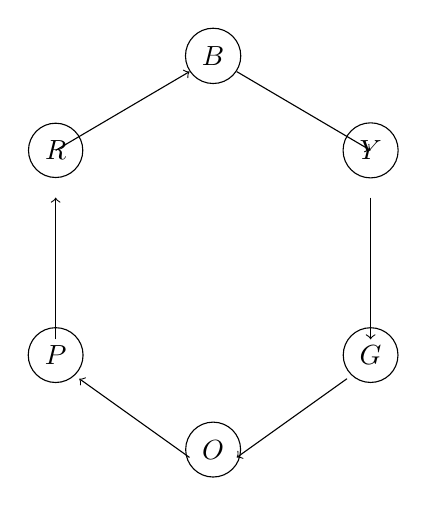
\begin{tikzpicture}[scale=1.0]
\draw[->] (0,2) -- (1.7,3);
\draw[->] (2.3,3) -- (4,2);
\draw[->] (4,1.4) -- (4,-0.4);
\draw[->] (3.7,-0.9) -- (2.3,-1.9);
\draw[->] (1.7,-1.9) -- (0.3,-0.9);
\draw[->] (0,-0.4) -- (0,1.4);

\node[draw,circle] at (0,2) {$R$};
\node[draw,circle] at (2,3.2) {$B$};
\node[draw,circle] at (4,2) {$Y$};
\node[draw,circle] at (4,-0.6) {$G$};
\node[draw,circle] at (2,-1.8) {$O$};
\node[draw,circle] at (0,-0.6) {$P$};
\end{tikzpicture}
\caption{At the moment Susskind says ``I'm going to draw this law as a diagram,'' the board still shows earlier probability notation on the left and the six-step update list on the right. Below it we redraw the same law as a closed cycle.}
\end{figure}

Assume that each update takes the same discrete time interval. Then if we sample the system at an unknown instant, without knowing where on the cycle it began, the probabilities are
\begin{equation}
p(R)=p(B)=p(Y)=p(G)=p(O)=p(P)=\frac16.
\end{equation}
The system spends one sixth of its time in each state, and that is the whole reason for the uniform distribution.

The lecture then strengthens the point by changing the order of the cycle while keeping the property that each color is visited once per period. The conclusion remains the same. The probability \(1/6\) does not depend on knowing the microscopic starting point, and it does not even depend on the detailed ordering of the cycle. It depends only on the orbit structure: one closed cycle, equal time per step, one visit per state.

\subsection{Question \& Answer}

\paragraph{Question.} If the system is not symmetric, why can each state still have probability \(1/6\)?

\paragraph{Answer.} Because the probability here is not being assigned by the shape of the object. It is being assigned by the time spent in each state. The lecture is very explicit on this point. If the system moves deterministically through a single six-step cycle, and if we are ignorant of the starting moment, then a random flash snapshot has to weight the six time-slots equally. The relevant symmetry is therefore a symmetry of the orbit in time, not a symmetry of the die in space.

\section{Cycles, Conserved Quantities, And Two Connected Systems}

The next move complicates the state space in exactly the right way. The six states need not lie on one big cycle. They may split into disconnected cycles. Suppose, for example, that one law produces the three-cycle
\begin{equation}
R\to B\to G\to R
\end{equation}
and another disconnected three-cycle
\begin{equation}
P\to Y\to O\to P.
\end{equation}
If we know the system is on the first cycle, then
\begin{equation}
p(R)=p(B)=p(G)=\frac13,
\qquad
p(P)=p(Y)=p(O)=0.
\end{equation}
If we know it is on the second cycle, the reverse is true.

But now a new issue appears. Dynamics alone does not tell us the probability of being on the first cycle rather than the second. That extra information has to come from elsewhere. Susskind's way of saying this is that one must supply some other probability, some prior information that chooses between the cycles. In the lecture the cycles are labeled \(+1\) and \(-1\), and that label is interpreted as a conserved quantity. It could be a toy quantity, but it could just as well be energy.

So let \(p_{+}\) be the prior probability for the \(+1\) cycle and \(p_{-}\) for the \(-1\) cycle, with
\begin{equation}
p_{+}+p_{-}=1.
\end{equation}
Then the probabilities inside each sector are still uniform, but the overall state probabilities are
\begin{equation}
p(R)=p(B)=p(G)=\frac{p_{+}}{3},
\qquad
p(P)=p(Y)=p(O)=\frac{p_{-}}{3}.
\end{equation}

This is the first real appearance of a conservation law. A conserved quantity partitions the space of states into sectors, and deterministic motion remains trapped inside one sector. Once that is so, there are really two distinct questions. First: within a given sector, how is time distributed among the available states? Second: what is the prior probability of being in that sector at all? The first question is answered by cycling. The second is not.

The lecture even remarks that the cycles need not have the same size. One sector might contain four states while another contains two. That changes the probabilities within a sector, but it does not change the logic. A conserved quantity partitions the configuration space, and statistical mechanics must somehow determine the relative weights of the sectors.

This is the bridge to honest energy. A single closed box may be treated as a universe unto itself, with a conserved energy. Two isolated boxes have two separately conserved energies. But if the boxes are connected by a narrow passage so that energy can pass between them, then only the total energy is conserved, and the new statistical question is forced upon us: given the total energy, what is the probability that one subsystem has a specified share?

\begin{figure}[h]
\centering

\includegraphics[width=0.78\textwidth]{lecture_01_figure_03.png}

\begin{tikzpicture}[scale=0.95]
\draw (-4,2.2) -- (-4,-1.4);
\draw (-4,2.2) -- (-0.6,2.2);
\draw (-4,-1.4) .. controls (-2.6,-1.9) and (-1.5,-1.9) .. (-0.6,-1.4);
\draw (-0.6,2.2) -- (-0.6,0.8);
\draw (-0.6,-1.4) -- (-0.6,-0.1);

\draw (0.6,2.0) -- (4.1,2.0);
\draw (4.1,2.0) -- (4.1,-1.6);
\draw (4.1,-1.6) -- (0.6,-1.6);
\draw (0.6,2.0) -- (0.6,0.8);
\draw (0.6,-0.1) -- (0.6,-1.6);

\draw (-0.6,0.8) -- (0.6,0.8);
\draw (-0.6,-0.1) -- (0.6,-0.1);
\end{tikzpicture}
\caption{The lecture's sketch of two connected subsystems. Once the two parts can exchange energy, the statistical problem becomes the problem of how a fixed total energy is distributed between them.}
\end{figure}

If the two boxes are equal, one expects equal energy on average. But that is only the first moment of the problem. The real question is the distribution itself. This is exactly where the lecture wants us: dynamics has produced sectors, conservation laws have appeared, and now the statistical question is how to assign probabilities to those sectors in a physically meaningful way.

\section{Good Laws, Bad Laws, And The Minus First Law}

At this point Susskind takes a step that is diagnostic rather than constructive. Before deciding how to assign probabilities, he asks what kinds of laws are even allowed. Some laws are bad, not in a moral sense, but in the sense that physics forbids them.

The prototype is the rule that sends every state to the same state:
\begin{align}
R &\to R, & B &\to R, & Y &\to R, \nonumber\\
G &\to R, & O &\to R, & P &\to R. \label{eq:all_to_red}
\end{align}
This law predicts the future in a trivial way. Wherever you are, next you are at red. But it destroys the past. If the present state is red, you can no longer reconstruct where you came from. Distinctions between states have been erased.

That is what Susskind means by loss of information. He gives the principle a name of his own: the minus first law of physics. Information is never lost. Differences between states propagate with time. A good law is therefore one in which every state has one incoming arrow and one outgoing arrow. In discrete language that is the mark of reversibility: one arrow tells you where you are going, the other tells you where you came from.

The lecture then reformulates the same point probabilistically. Suppose that at some moment \(M\) out of \(N\) states carry equal nonzero probability \(1/M\), while the remaining states have probability zero. Under a good law, the occupied states may reshuffle, but there will later still be exactly \(M\) occupied states, each with probability \(1/M\). Under a bad law such as \eqref{eq:all_to_red}, that number can collapse. Distinct possibilities are merged. This observation is the bridge from information conservation to entropy.

In continuum mechanics the corresponding theorem is Liouville's theorem. A region of occupied phase space may stretch, shear, and fold, but its phase-space volume is preserved. More than that, a probability distribution that is initially uniform on the occupied region remains uniform on the evolved region. The discrete rule ``\(M\) occupied states stay \(M\) occupied states'' and the continuous rule ``occupied phase-space volume is preserved'' are the same principle in two different languages.

\subsection{Question \& Answer}

\paragraph{Question.} Why does friction not really violate conservation of information?

\paragraph{Answer.} Because friction only looks like a fundamental information-destroying law when we describe too few degrees of freedom. Susskind's schematic example is a viscous-drag equation of the form
\begin{equation}
m\ddot x=-\gamma \dot x.
\end{equation}
Taken literally as a fundamental law for a closed many-particle system, such an equation would be disastrous: every particle would drift toward rest, energy would disappear, and the system would evolve toward a simpler, less informative description. It would be the continuum analog of ``everything goes to red.''

But real friction is not that. When an eraser slows down on a table, the lost macroscopic motion is recorded in microscopic variables of the eraser, the table, and the surrounding air. If we look only at the visible coordinate \(x\) and its conjugate momentum, the distribution seems to contract. In the full higher-dimensional phase space, however, the distribution spreads into hidden directions. The apparent collapse is a projection. Liouville volume is preserved in the full closed system even though it is not preserved in the macroscopic variables we happen to be watching.

That is the point of the example. The lecture does not need the exact drag coefficient. It needs the conceptual lesson: apparent irreversibility at the coarse level is compatible with information conservation at the microscopic level.

\section{The First Law And The Additivity Caveat}

After the minus first law, Susskind deliberately skips the zeroth law and states the first law in its simplest possible form. Energy is conserved:
\begin{equation}
\frac{dE}{dt}=0.
\end{equation}
That is all the first law says for a closed system.

If the system is built from two weakly interacting parts, then the total energy is approximately additive,
\begin{equation}
E \approx E_1+E_2,
\end{equation}
and differentiation gives
\begin{align}
\frac{dE_1}{dt}+\frac{dE_2}{dt} &= 0, \\
\frac{dE_1}{dt} &= -\frac{dE_2}{dt}.
\end{align}
Susskind explicitly writes the second form to make the physical interpretation vivid: what leaves one subsystem enters the other.

He is equally explicit about the caveat. Exact additivity is not always true. If two bodies interact gravitationally, for example, the total energy is not merely the kinetic energy of one plus the kinetic energy of the other. There is also the potential energy of interaction, and it belongs to the pair rather than to either body separately.

Why then is additivity so useful in thermodynamics? Because in many large systems the interaction term is a surface effect while the bulk energy is a volume effect. If we divide a large body into blocks, the energy in a block scales with its volume, whereas the interaction between neighboring blocks scales with the contact area of their surfaces. For large enough blocks the interaction term is negligible by comparison, and the additive approximation becomes excellent. The first law is always true. The two-subsystem form is true when interaction energies are small enough to ignore.

This short section matters because it fixes the hierarchy of the lecture. Energy conservation is fundamental, but in this first lecture it is being inserted only after information conservation has been clarified. Entropy is then allowed to return in a sharper form.

\section{Entropy As A Measure Of Ignorance}

\subsection{Occupied States And The First Definition}

Now the lecture explicitly returns to entropy. Up to this point Susskind has defined it only in a special case, but he has already motivated the key ingredient: the number of states that are genuinely available to us given our incomplete knowledge.

Suppose there are \(N\) possible states altogether, but only \(M\) of them have nonzero probability, and suppose those \(M\) occupied states are equally likely. Then
\begin{equation}
p_i=\frac{1}{M}
\quad\text{for the occupied states,}
\qquad
p_i=0
\quad\text{for the others.}
\end{equation}
The entropy is defined by
\begin{equation}
S=\log M.
\end{equation}

This is already enough to capture the lecture's main idea. If \(M=N\), then all states are equally probable and our ignorance is maximal:
\begin{equation}
S_{\max}=\log N.
\end{equation}
If \(M=1\), then the system is known to be in one specific state and the entropy is zero.

Susskind keeps returning to the same interpretation: \(M\) measures ignorance. The bigger \(M\) is, the less we know. And because a good law only reshuffles occupied states without changing their number, \(M\) is conserved under exact microscopic evolution. In that sense entropy is conserved if we can follow the system perfectly.

But we usually cannot follow the system perfectly. We lose track of phases, timing, microscopic positions, and details of the dynamics. Then the entropy increases, not because the equations have destroyed information, but because our description has become coarser. That is why Susskind insists that entropy enters before temperature and, in a certain sense, before energy in the pedagogical order of the lecture. It is the measure of our statistical ignorance.

\subsection{General Probability Distributions}

The lecture then says, in effect: we are not finished with entropy. The special rectangular distribution is too narrow a case. Most probability distributions are not flat on their occupied set. To show what a more general situation looks like, Susskind draws the states schematically along a horizontal axis and plots the corresponding probabilities on the vertical axis.

\begin{figure}[h]
\centering

\includegraphics[width=0.74\textwidth]{lecture_01_figure_05.png}

\begin{tikzpicture}[scale=0.9]
\draw[->] (-4.2,0) -- (4.4,0);
\draw[->] (-4,0) -- (-4,3.2);
\node at (-4.45,3.0) {$p_i$};

\draw (-3.6,0.1) -- (-3.6,-0.1);
\draw (-3.1,0.1) -- (-3.1,-0.1);
\draw (-2.6,0.1) -- (-2.6,-0.1);
\draw (-2.1,0.1) -- (-2.1,-0.1);
\draw (-1.6,0.1) -- (-1.6,-0.1);
\draw (-1.1,0.1) -- (-1.1,-0.1);
\draw (-0.6,0.1) -- (-0.6,-0.1);
\draw (-0.1,0.1) -- (-0.1,-0.1);
\draw (0.4,0.1) -- (0.4,-0.1);
\draw (0.9,0.1) -- (0.9,-0.1);
\draw (1.4,0.1) -- (1.4,-0.1);
\draw (1.9,0.1) -- (1.9,-0.1);
\draw (2.4,0.1) -- (2.4,-0.1);
\draw (2.9,0.1) -- (2.9,-0.1);
\draw (3.4,0.1) -- (3.4,-0.1);

\draw plot[smooth] coordinates {
(-3.7,0.18) (-3.0,0.25) (-2.4,0.55) (-1.7,1.25)
(-1.0,2.05) (-0.4,2.45) (0.0,2.3) (0.5,1.95)
(1.2,1.35) (1.9,0.8) (2.7,0.42) (3.5,0.18)
};

\draw (-1.9,-0.15) -- (-1.9,-0.45);
\draw (1.8,-0.15) -- (1.8,-0.45);
\draw (-1.9,-0.45) -- (1.8,-0.45);
\node at (-0.05,-0.8) {$M$};
\end{tikzpicture}
\caption{The lecture's schematic probability graph over discrete state labels. The picture is qualitative, but its purpose is precise: a narrower distribution represents fewer significantly occupied states and therefore less entropy, while a broader one represents more and therefore more entropy.}
\end{figure}

The definition that handles the general case is
\begin{equation}
S=-\sum_i p_i\log p_i.
\end{equation}
Susskind immediately remarks that this is minus the average of \(\log p_i\). That is why the earlier expectation-value machinery mattered. The new entropy formula is built directly out of it.

The minus sign is not mysterious. Probabilities are numbers less than \(1\), so their logarithms are negative. The overall minus sign is there so that entropy comes out positive in the cases of interest. The lecture then checks the formula against the original \(S=\log M\).

If \(p_i=1/M\) on the occupied states and \(p_i=0\) elsewhere, then the states of zero probability contribute nothing because
\begin{equation}
\lim_{p\to 0^+} p\log p = 0.
\end{equation}
For the occupied states,
\begin{align}
S
&= -\sum_{\text{occupied }i}\frac{1}{M}\log\!\left(\frac{1}{M}\right) \\
&= -M\left[\frac{1}{M}\log\!\left(\frac{1}{M}\right)\right] \\
&= -\log\!\left(\frac{1}{M}\right) \\
&= \log M.
\end{align}
So the new definition reduces exactly to the old one in the special case where it must.

This is the moment at which the lecture gives its qualitative interpretation of the graph. The narrower the distribution, the smaller the entropy. The broader the distribution, the larger the entropy. The later frame below simply reinforces that visual point by drawing attention to the width marker \(M\).

\begin{figure}[h]
\centering

\includegraphics[width=0.72\textwidth]{lecture_01_figure_06.png}
\caption{A later frame of the same graph. The lecturer's gesture singles out the spread of the distribution, which is exactly the feature the surrounding discussion interprets as controlling the entropy.}
\end{figure}

\subsection{Coins As Explicit Examples}

The lecture now returns once more to coins, because they let us see the definitions work in explicit examples. To keep the notation straight, let \(n\) denote the number of coins, and let \(N\) denote the total number of states of the \(n\)-coin system. Then
\begin{equation}
N=2^n.
\end{equation}

If we know nothing at all, then every one of the \(2^n\) states is equally probable. Therefore
\begin{equation}
S=\log(2^n)=n\log 2.
\end{equation}
This is the maximal entropy of the \(n\)-coin system.

If the microscopic state is known completely, then only one state has nonzero probability. In that case
\begin{equation}
S=0.
\end{equation}
Perfect knowledge means zero entropy.

The more interesting example is the one Susskind works through with the class. Suppose all \(n\) coins are heads except for exactly one tail, but we do not know which coin is tails. Then there are exactly \(n\) states with nonzero probability, all equally weighted, and therefore
\begin{equation}
S=\log n.
\end{equation}
This example matters because it shows that with natural logarithms entropy is not, in general, an integer multiple of \(\log 2\).

The lecture also addresses the base of the logarithm. In these notes, as in the lecture, \(\log\) means the natural logarithm. In information theory one often uses base \(2\), in which case the entropy of a completely unknown single coin is \(1\) bit. The choice of base changes only an overall numerical factor. It does not change the structure of the theory.

\subsection{Continuous Phase Space}

The lecture then enlarges the whole discussion from discrete state spaces to classical phase space. A microscopic state is now a point specified by coordinates and momenta. Susskind uses both \(x\) and \(q\) verbally for coordinates; we will simply write the state space abstractly as phase space \(\Gamma\), and we will denote the phase-space volume element by \(d\Gamma\).

Suppose first that the probability distribution is uniform on some occupied blob of phase space and zero outside. Then the continuous analog of counting occupied states is measuring the phase-space volume of the occupied region. The entropy is defined by
\begin{equation}
S=\log V_{\Gamma},
\end{equation}
where \(V_{\Gamma}\) is the phase-space volume of the blob.

For a general probability density \(P\) on phase space, the normalization condition is
\begin{equation}
\int d\Gamma\,P = 1,
\end{equation}
and the entropy becomes
\begin{equation}
S=-\int d\Gamma\,P\log P.
\end{equation}
This is exactly the continuous analog of the discrete formula. One simply replaces the sum over discrete states by an integral over phase space.

Susskind's interpretation remains the same. In first conceptual approximation, the entropy measures the logarithm of the volume of the probability blob. More generally, it measures how spread out the probability density is in phase space. It is still a property of a probability distribution, not a property of a microscopic state by itself. A single exact microstate has no entropy except in the trivial sense that the entropy of the corresponding probability distribution is zero.

\subsection{Correlation And Additivity}

The lecture closes by sharpening the interpretation of entropy through correlation. If we truly know nothing about a collection of coins, then measuring one coin tells us nothing about the others. The remaining probabilities are unchanged. That is the uncorrelated case.

But if we know that exactly one coin among \(n\) is tails, then a measurement of one coin changes our knowledge of the rest. If the measured coin is tails, the others are certainly heads. If the measured coin is heads, then the probability that any given remaining coin is the tail becomes
\begin{equation}
p(\text{tail on a given remaining coin}\mid \text{measured head})
=
\frac{1}{n-1}.
\end{equation}
That is Susskind's definition of correlation: measuring one thing changes the probability distribution for another thing.

This links directly back to the earlier discussion of conserved sectors. Once we determine a conserved quantity, the admissible set of states changes, and so the probability distribution changes with it. Correlation is therefore not an ornamental afterthought. It is part of the central logic of statistical mechanics: knowledge about one part of a system can constrain what remains possible elsewhere.

Entropy is additive when there is no correlation. For uncorrelated subsystems the total entropy is the sum of the entropies of the parts. When there are correlations, additivity fails in exactly the way one would expect: some of the ignorance in one subsystem is no longer independent of the ignorance in another.

The audience then asks about the relation to information theory. Susskind's answer is that the Boltzmann and Shannon entropies are the same formula up to the base of the logarithm and a sign convention. What is called entropy here is therefore a measure of lack of information. It is not the Heisenberg uncertainty principle. The lecture is explicit on that point: the entropy under discussion concerns probabilistic ignorance encoded in a mixed distribution over states, not the distinct quantum uncertainty attached to a pure state.

\section{Summary}

The first lecture unfolds in a very deliberate order. Statistical mechanics is first justified as a deep and central subject. Then probability is reviewed as the language of incomplete knowledge. Then deterministic laws are shown to generate probabilities through ignorance of the starting point. Then conservation laws partition the state space, and the conservation of information is elevated to the minus first law. Only after that does the lecture state the first law and return to entropy.

Entropy begins as
\begin{equation}
S=\log M,
\end{equation}
the logarithm of the number of equally probable occupied states. It then broadens to
\begin{equation}
S=-\sum_i p_i\log p_i,
\end{equation}
and finally to the continuous phase-space form
\begin{equation}
S=-\int d\Gamma\,P\log P.
\end{equation}
In every case the meaning is the same: entropy is not a bare property of a microscopic state; it is a measure of our probabilistic ignorance, organized over the space of possible states.

That is the real achievement of the lecture. By the end, entropy has been made concrete enough to calculate, broad enough to survive the passage from discrete to continuous systems, and precise enough to prepare the next step, where temperature and the Boltzmann distribution will enter.